\begin{figure*}[t!]
  \centering
  \subfigure[BERT-Base pretraining seq128]{
    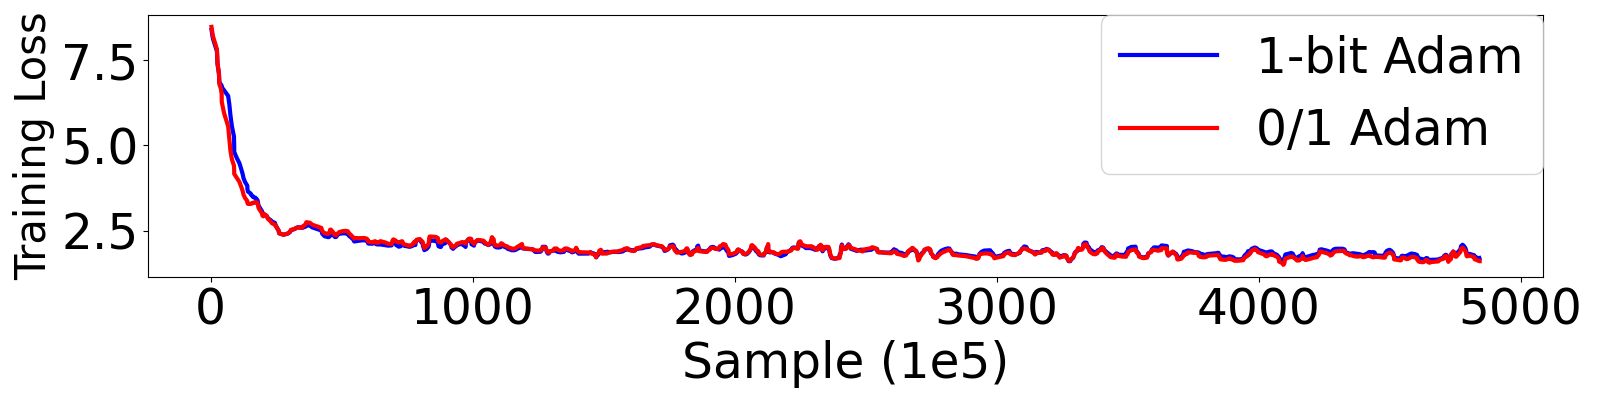
\includegraphics[width=0.5\textwidth]{./sections/figure/v3_base_sample.png}
    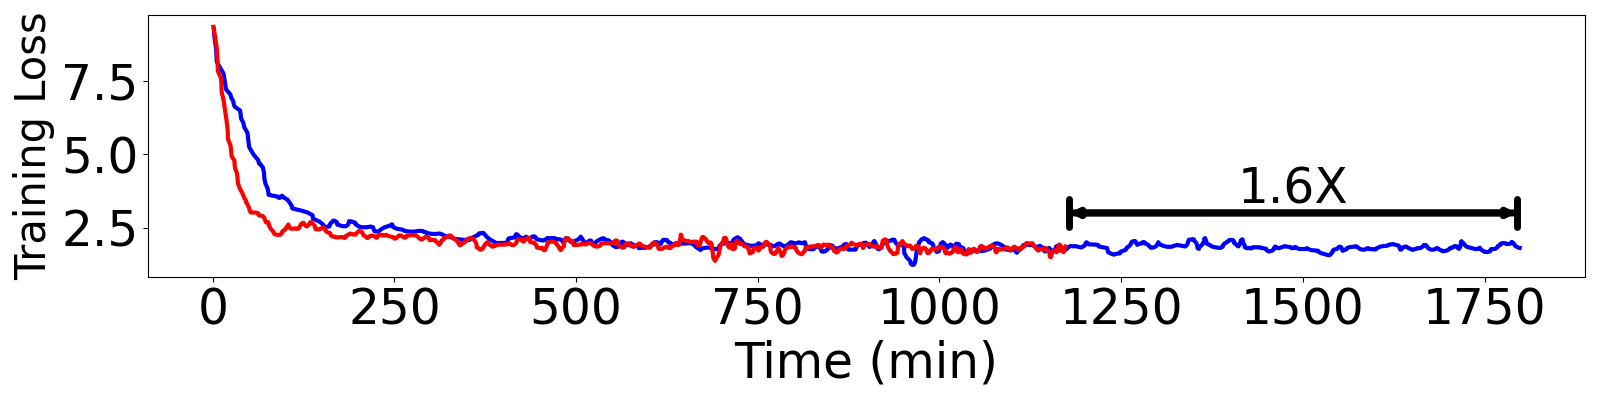
\includegraphics[width=0.5\textwidth]{./sections/figure/v3_base_time.png}
    }
  \subfigure[BERT-Large pretraining seq128]{
    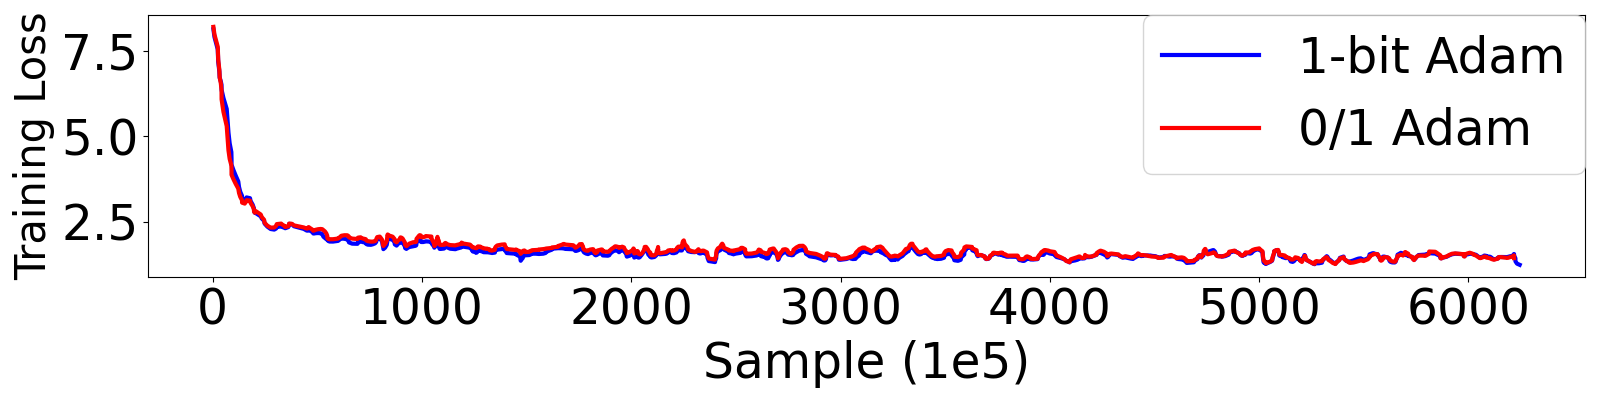
\includegraphics[width=0.5\textwidth]{./sections/figure/v3_large_sample.png}
    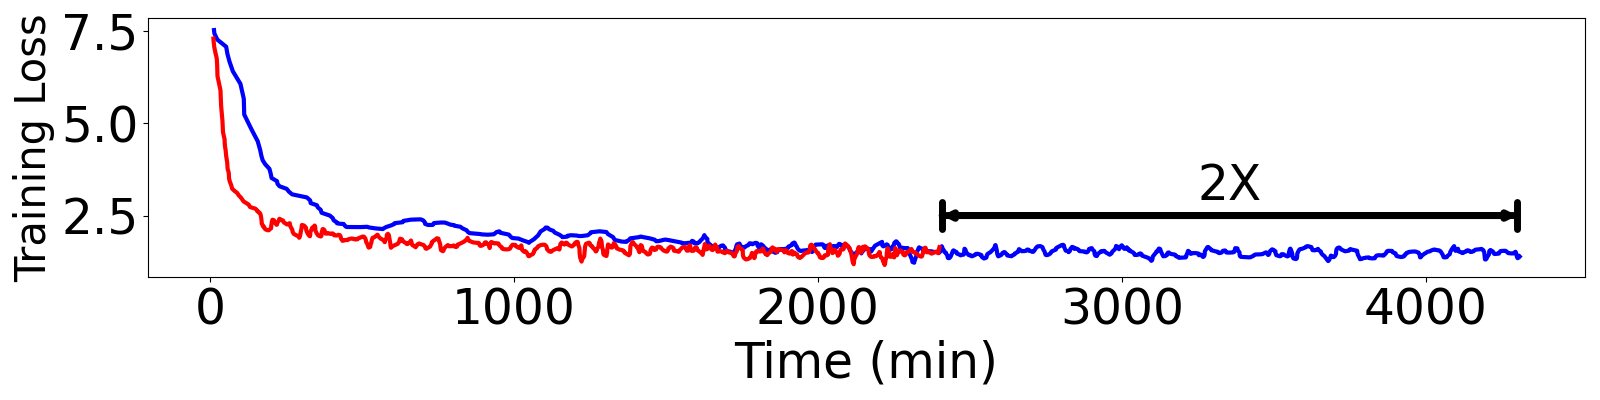
\includegraphics[width=0.5\textwidth]{./sections/figure/v3_large_time.png}
    }
  \subfigure[Resnet18 on ImageNet]{
    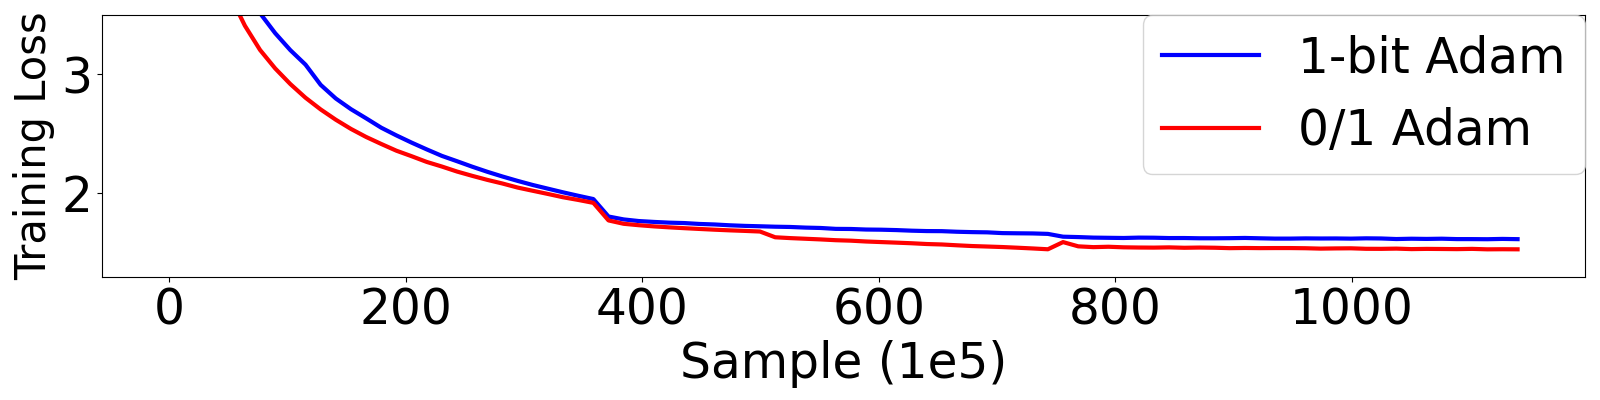
\includegraphics[width=0.5\textwidth]{./sections/figure/v3_imagenet_sample.png}
    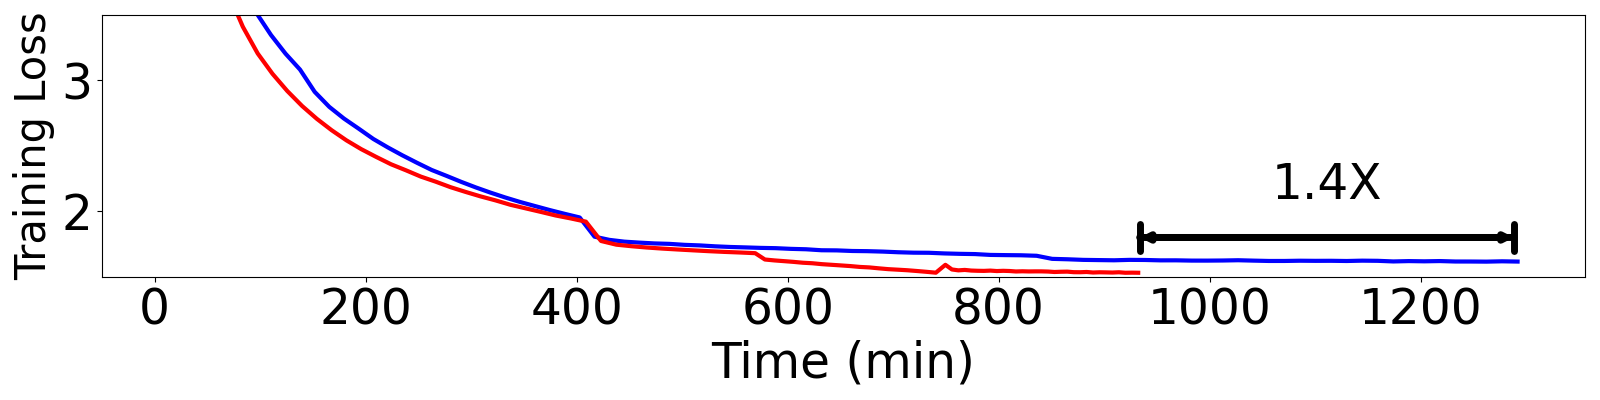
\includegraphics[width=0.5\textwidth]{./sections/figure/v3_imagenet_time.png}
    }
    \caption{Sample-wise and time-wise convergence for BERT-Base/Large pre-training sequence length 128 and Resnet18 pretraining on ImageNet using 128 GPUs on the Ethernet cluster.}
    \label{exp:fig:convergence}
\end{figure*}


\begin{figure*}[t!]
  \centering
  \subfigure[BERT-Base (Ethernet) batch size=4096]{
    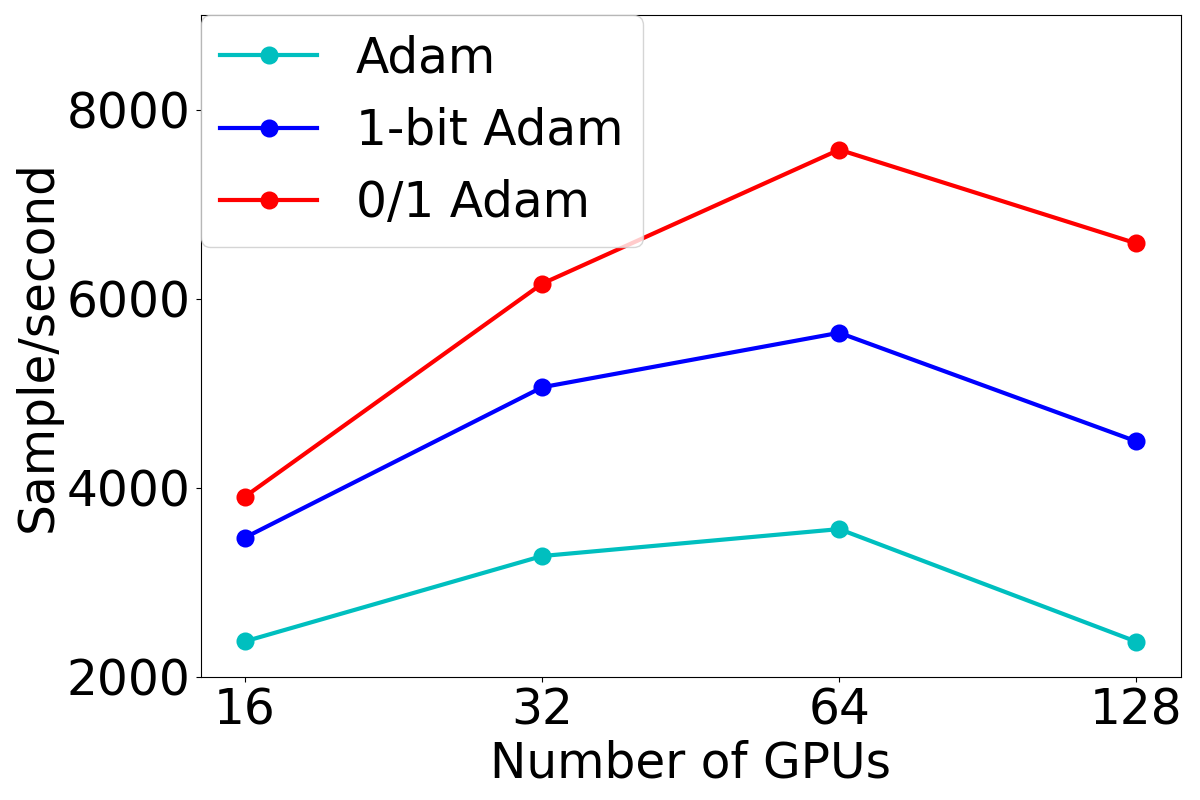
\includegraphics[width=0.22\textwidth]{./sections/figure/throughput_base.png}
    }
  \subfigure[BERT-Large (Ethernet) batch size=4096]{
    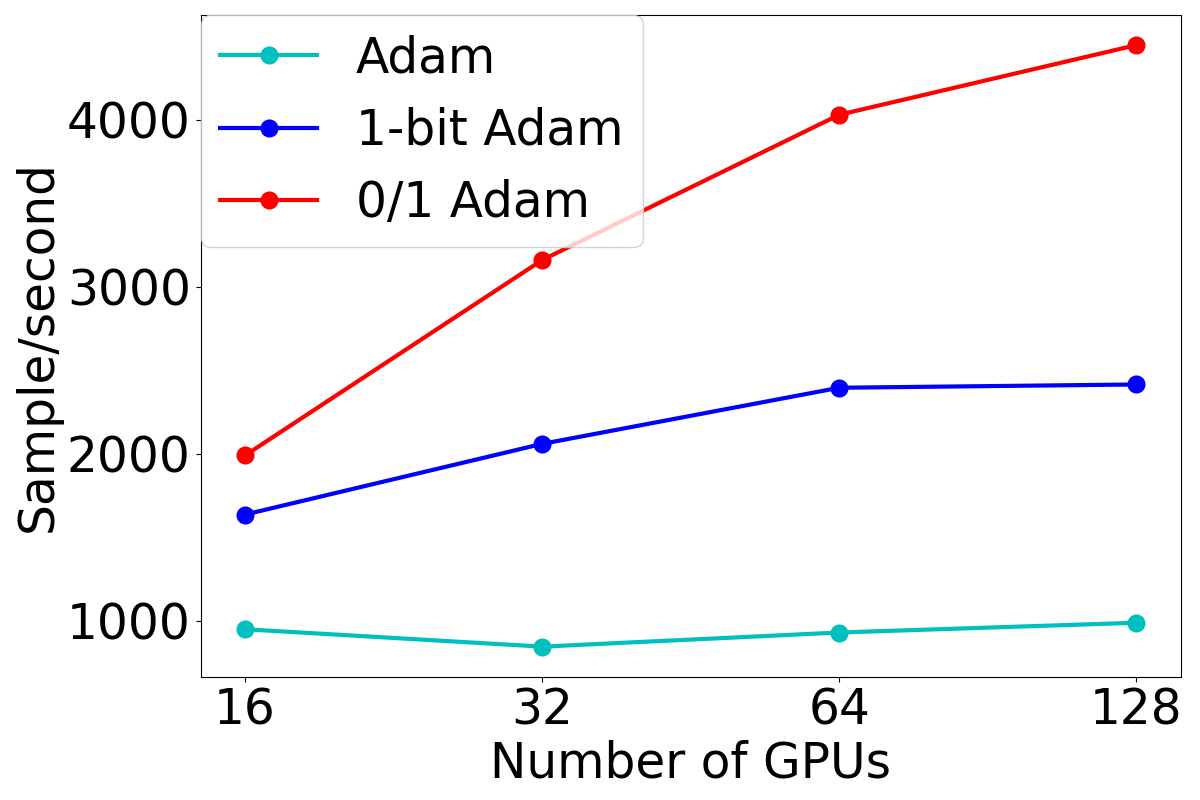
\includegraphics[width=0.22\textwidth]{./sections/figure/throughput_large.png}
    \label{exp:fig:throughput:bertlarge:eth}
    }
  \subfigure[BERT-Large (InfiniBand) batch size=4096]{
    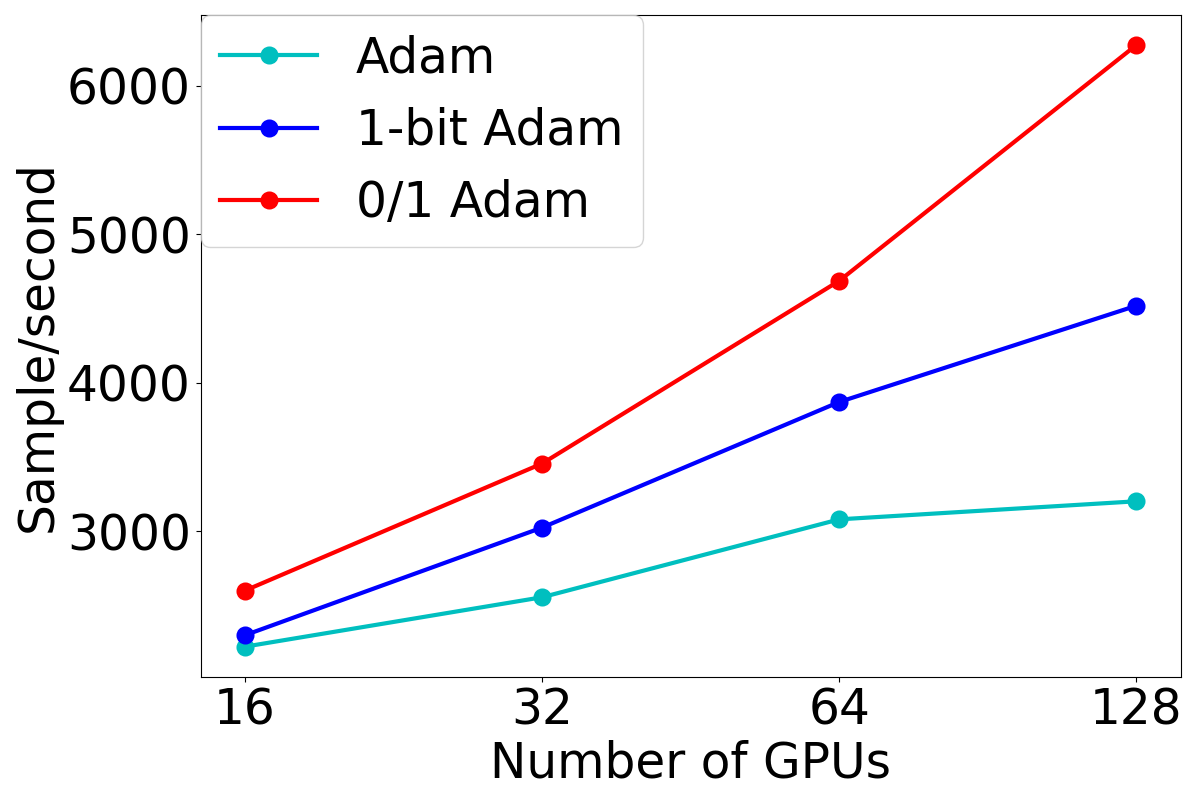
\includegraphics[width=0.22\textwidth]{./sections/figure/throughput_ib_large.png}
    \label{exp:fig:throughput:bertlarge:ib}
    }
  \subfigure[ImageNet (Ethernet) batch size=256]{
    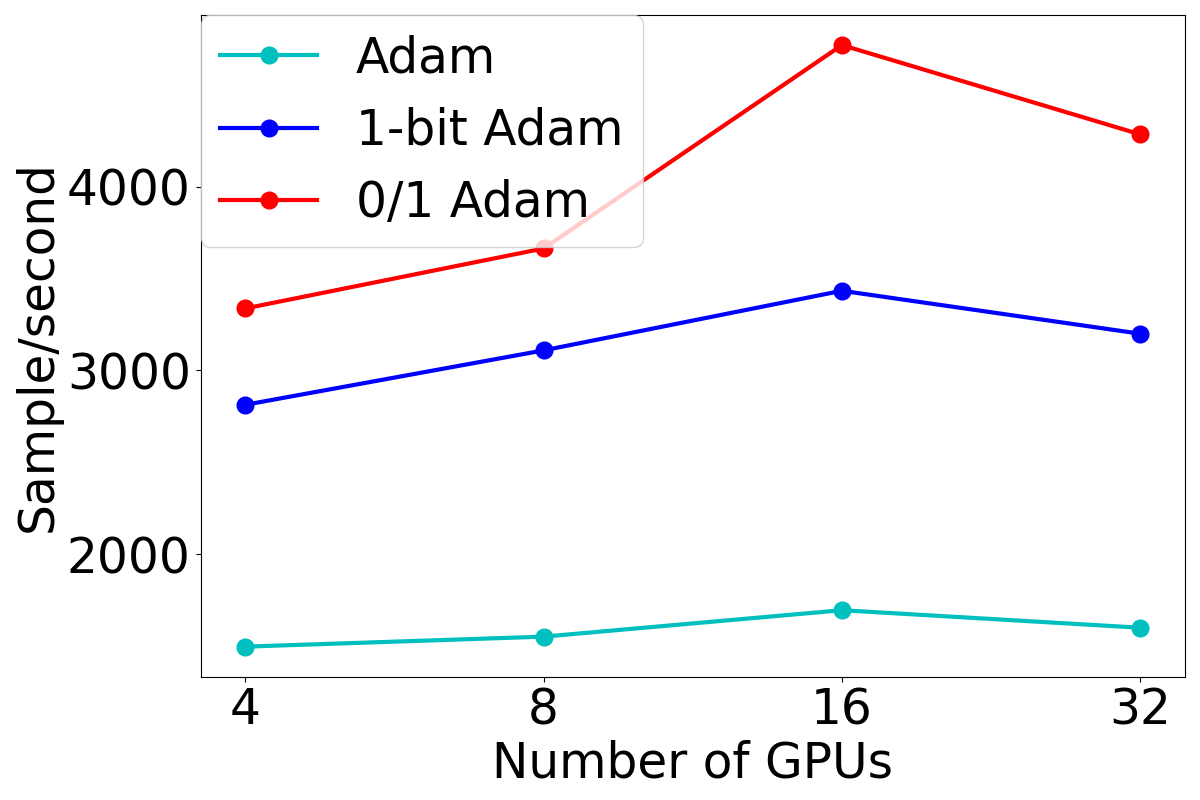
\includegraphics[width=0.22\textwidth]{./sections/figure/throughput_imagenet.png}
    }
  \caption{End-to-end average throughput for BERT-Base/Large pre-training sequence length 128 and Resnet18 pretraining on ImageNet using 128 V100 GPUs on the Ethernet/InfiniBand cluster. Note that since for ImageNet, both batch size (256) and model (Resnet18) are small compared to BERT, and its parallelism speed up will be limited if applied to the same large system on BERT (128 GPUs). And so we test it for 4 to 32 GPUs in Figure (d).}
  \label{exp:fig:throughput}
\end{figure*}

\section{Experiments}
\label{sec:experiment}
In this section we evaluate the performance of {\myalgo} over several large-scale model training tasks comparing with baselines (1-bit Adam \citep{tang20211} and original Adam \citep{kingma2014adam}). Since \citet{tang20211} already demonstrated that 1-bit Adam has similar statistical results to Adam, we omit the comparison of end-to-end model accuracy to Adam for brevity.
Throughout the experiments, we enable FP16 training for all the tasks following \citep{tang20211}. That makes the full-precision communication (including Adam, full-precision stage in 1-bit Adam and full-precision AllReduce in {\myalgo}) use 16-bit per number. We use the 1-bit compressor (Equation~(\ref{equa:1bitcompression})) in {\myalgo}.

\begin{table*}[t]
  \centering
  \newcommand{\colspc}{\hspace*{0.35em}}
  \caption{GLUE development set results. BERT-Base/Large(original) results are from \citep{devlin2018bert}. BERT-Base/Large(1-bit Adam) results are from \citep{tang20211}. The scores are the median scores over 10 runs with different seeds, and are obtained on the checkpoints trained by both sequence 128 and sequence 512 datasets.}
  \label{exp:table:glue}
  \begin{tabular}{@{\colspc}l@{\colspc}c@{\colspc}c@{\colspc}c@{\colspc}c@{\colspc}c@{\colspc}c@{\colspc}c@{\colspc}c@{\colspc}c@{\colspc}}
  \hline  
  & RTE & MRPC & STS-B & CoLA & SST-2 & QNLI & QQP & MNLI-(m/mm) & Avg Score\\
  \hline  
  BERT-Base(Original) & 66.4 & 84.8 & 85.8 & 52.1 & 93.5 & 90.5 & 89.2 & 84.6/83.4 & 81.1 \\
  BERT-Base(1-bit Adam) & 69.0 & 84.8 & 83.6 & 55.6 & 91.6 & 90.8 & 90.9 & 83.6/83.9 & 81.5 \\
  BERT-Base({\myalgo}) & 69.7 & 85.1 & 84.9 & 54.4 & 91.9 & 90.3 & 90.7  & 83.7/83.7 & 81.6 \\
  \hline
  BERT-Large(Original) & 70.1 & 85.4 & 86.5 & 60.5 & 94.9 & 92.7 & 89.3 & 86.7/85.9 & 83.6\\
  BERT-Large(1-bit Adam) & 70.4 & 86.1 & 86.1 &  62.0 & 93.8 & 91.9 & 91.5 & 85.7/85.4  & 83.7\\
  BERT-Large({\myalgo}) & 71.7 & 86.2 & 86.9 & 59.9 & 93.2 & 91.6 & 91.4 & 85.6/85.6  & 83.6\\
  \hline
  \end{tabular}
\end{table*}

\begin{table}[t]
  \centering
  \caption{The first column shows Top1 accuracy on ImageNet of Resnet at the end of epoch 90 from different algorithms. The original accuracy is provided by Pytorch pretrained model library \citep{pytorchTorchvisionmodelsx2014}. For the other two algorithms, the accuracy is the highest score over 3 runs. The other two columns shows zero-shot evaluation of the trained GPT-2 on WikiText-103 and LAMBADA datasets, the evaluation methodology follows \citep{shoeybi2019megatron}. The number for Adam is obtained from \citep{li2021curriculum}.}
  \label{exp:table:imagenet}
  \begin{tabular}{lccccccccc}
  \hline  
  & ImageNet Top1 Acc. $\uparrow$ & WikiText Perplexity $\downarrow$ & LAMBADA Acc. $\uparrow$ \\
  \hline 
  Original Adam & 69.76 & 27.78 & 33.19 \\
  1-bit Adam & 69.93 & 28.37 & 33.21 \\
  {\myalgo} & 69.88 & 28.07 & 33.51 \\
  \hline
  \end{tabular}
\end{table}

\textbf{Experimental details.}
We adopt the following tasks for the evaluation: BERT-Base ($L=12$, $H=768$, $A=12$, $110M$ params) and BERT-Large ($L=24$, $H=1024$, $A=16$, $340M$
params) pre-training, training Resnet18 ($12M$ params) on ImageNet \citep{he2016deep} and GPT-2 pre-training. For BERT model, we use the same dataset as \citep{devlin2018bert}, which is a concatenation of Wikipedia and BooksCorpus with 2.5B and 800M words respectively. We use the GLUE fine-tuning benchmark \citep{wang2018glue} to evaluate the convergence of the BERT models trained by different algorithms. For ImageNet, we adopt ImageNet-1k dataset, which contains 1.28M images for training and 50K images for validation \citep{deng2009imagenet}.
For GPT-2 we adopt the model from its original paper \citep{radford2019better}, which contains 117M parameters (48 layers, 1600 hidden size, 25 attention heads). For training data, we adopt the same dataset blend as in \citep{shoeybi2019megatron}: Wikipedia \citep{devlin2018bert}, CC-Stories \citep{trinh2018simple}, RealNews \citep{zellers2019defending}, and OpenWebtext \citep{radford2019better}. Other details including learning rate schedules, hyperparameters can be found in Appendix~\ref{appendix:sec:exp}.

\textbf{Hardware.}
We evaluate two clusters: one with 4 NVIDIA V100 GPUs per node and 40 Gigabit Ethernet inter-node network (2.7 Gbps effective bandwidth); the other one with 8 V100 GPUs per node and 100 Gigabit InfiniBand EDR inter-node network (close to theoretical peak effective bandwidth). We use 4 to 128 GPUs for BERT and ImageNet pretraining tasks to measure {\myalgo}'s performance gain.
We use 64 GPUs for GPT-2 pre-training.
Additionally, for ImageNet training we apply the accelerated data loading technique from lmdb\footnote{\url{https://github.com/xunge/pytorch_lmdb_imagenet}}.

% \minjia{If space is an issue, you can move the detailed hyperparameter settings to the appendix, and add something at the end of "dataset and models" that says "We mostly follow the settings from XXX... Please see Appendix XX for more training details." In that case, you can also change "Datasets and models" to "Experiment details". }

\textbf{Policy for $\mathcal{T}_{\*v}$ and $\mathcal{T}_{\*u}$ in {\myalgo}.}
We first illustrate our policy on $\mathcal{T}_{\*v}$.
Observing from our motivation study (Figure~\ref{fig:profile_bert_large}) that the variance difference in adjacent steps decreases roughly exponentially. Denote $k_j$ as the step where $j$-th variance update takes place, we select $\mathcal{T}_{\*v}$ such that, $k_{j+1} - k_j = 2^{\left\lfloor j/\kappa\right\rfloor}, \forall \kappa>0$.
We adopt $\kappa=16$ for all the three tasks.

Then we move on to discuss the policy for $\mathcal{T}_{\*u}$. Based on the derivation in Section~\ref{sec:algorithm}, the approximation noise from local step is proportional to the learning rate. And so if we denote $t_j$ as the step where $j$-th synchronization takes place, then our intuition is to increase $t_{j+1}-t_{j}$ roughly inversely proportional to the learning rate at $t_j$ so as to make the approximation noise bounded. 
For BERT-Base/Large pretraining, as illustrated before, the learning rate exponentially decreases by 0.99 every 520 steps after 12.5K linear increase warmup steps. So that we set $t_{j+1}-t_{j}=1$ for the first 12.5K steps and after that let it multiply by 2 every 32678 steps based on the calculation that the learning rate will decrease by half. Similarly, for ImageNet we set $t_{j+1}-t_{j}=1$ for the first 50050 steps (10 epochs) and after that let it multiply by 2 every 50050 steps (10 epochs).
We clip the interval at 16 in all the tasks. This corresponds to $H=16$ in Assumption~\ref{assume:localstep_bound}.Finally, since our theory in Section~\ref{sec:theory} indicates that approximation will be more accurate when the variance is frozen. So that we additionally stop updating variance when $t_{j+1}-t_{j} > 1$.

\subsection{Convergence Speed and Quality Analysis}
Figure~\ref{exp:fig:convergence} presents the sample-wise and time-wise convergence results for different algorithms with 128 GPUs on the Ethernet cluster. We find that {\myalgo} provides the same sample-wise convergence speed compared to the baseline, with up to 2$\times$ time-wise speed up. Table~\ref{exp:table:glue} summarizes the GLUE results using the checkpoints from our BERT pretraining experiments. {\myalgo} achieves similar end task accuracy compared to the numbers reported in previous work. \myalgo achieves faster training time than prior work because it reduces the communication overhead in distributed training by using both 1-bit quantizer to compress the communication volume (up to 32$\times$ reduction) and 1-bit AllReduce to reduce the expensive synchronization overhead for local steps in both warmup and non-warmup phases.  
Table~\ref{exp:table:imagenet} provides the ImageNet validation accuracy of trained models from different algorithms, and we find the final accuracy can achieve the reported accuracy from Pytorch library \citep{pytorchTorchvisionmodelsx2014}. For brevity, convergence comparison on GPT-2 is given in the Appendix~\ref{appendix:sec:exp}.
%\minjia{Shouldn't we add the description for the convergence speed and quality results for GPT-2 here as well? Also, given that we now claim one of the major difference between ours and 1-bit Adam is the study on autoregressive models like GPT, I feel we should have it in the main paper to better support the claim. Not sure if we have zero-shot evaluation results, but if so, it would be very helpful to add those as well.}

\begin{figure}[t!]
  \centering
  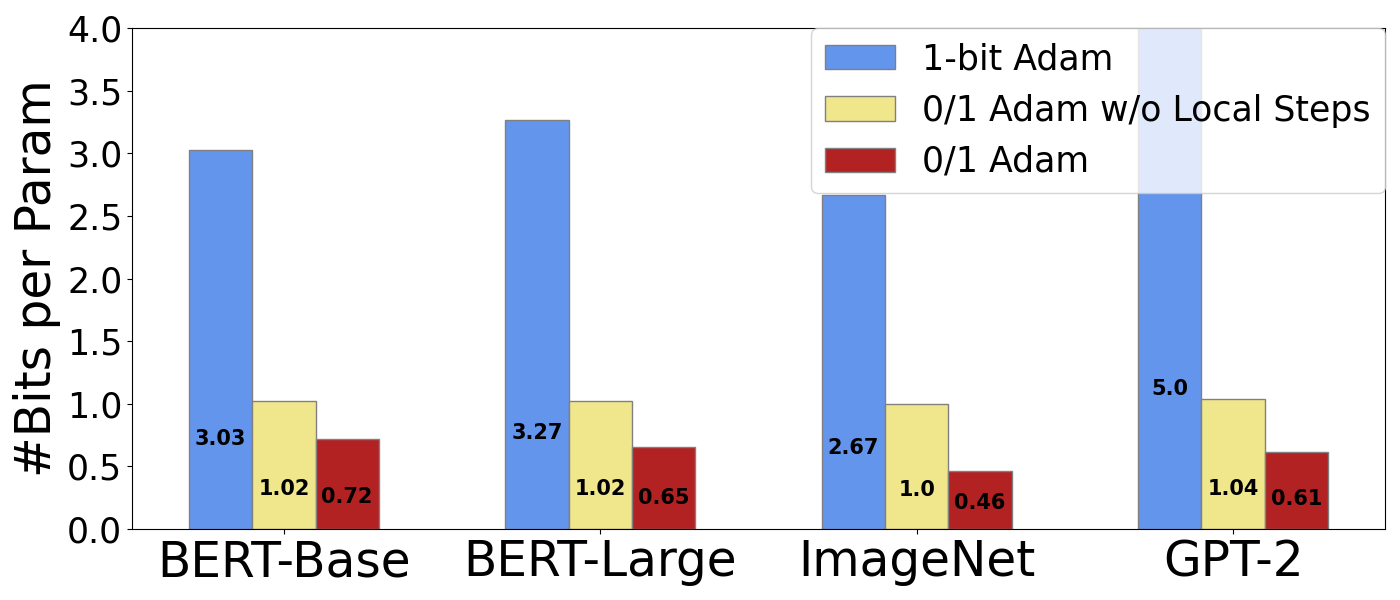
\includegraphics[width=0.45\textwidth]{./sections/figure/reduction_data_volume.png}
  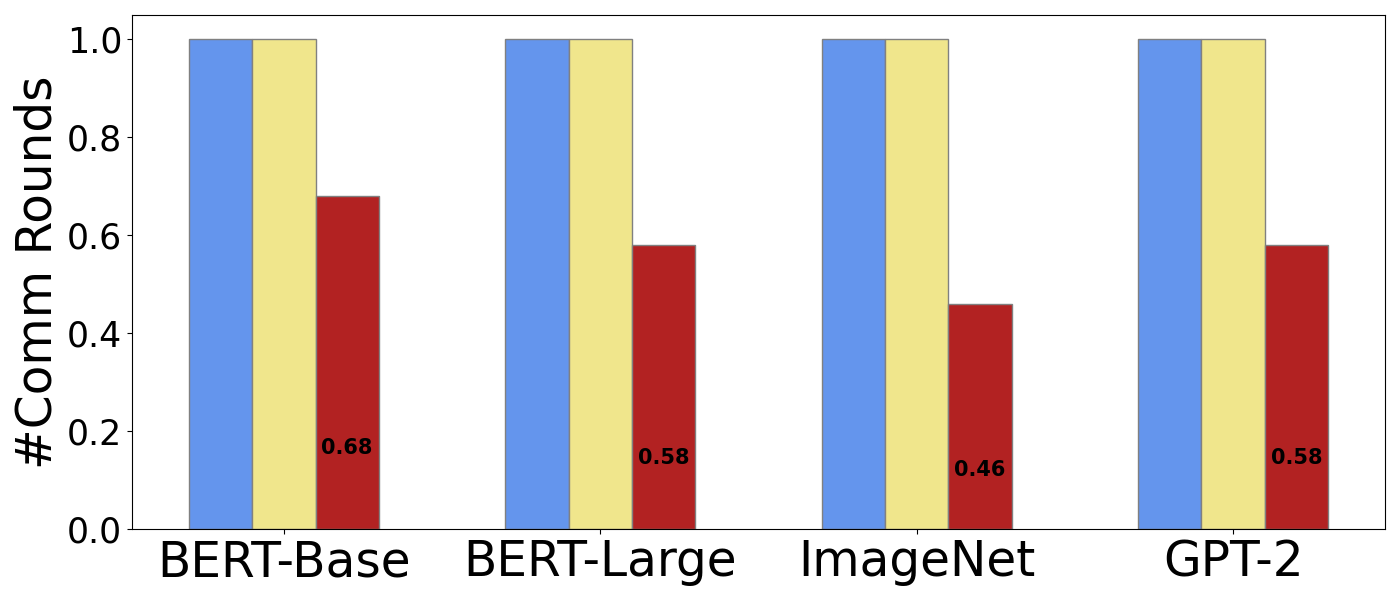
\includegraphics[width=0.45\textwidth]{./sections/figure/reduction_rounds.png}
  % 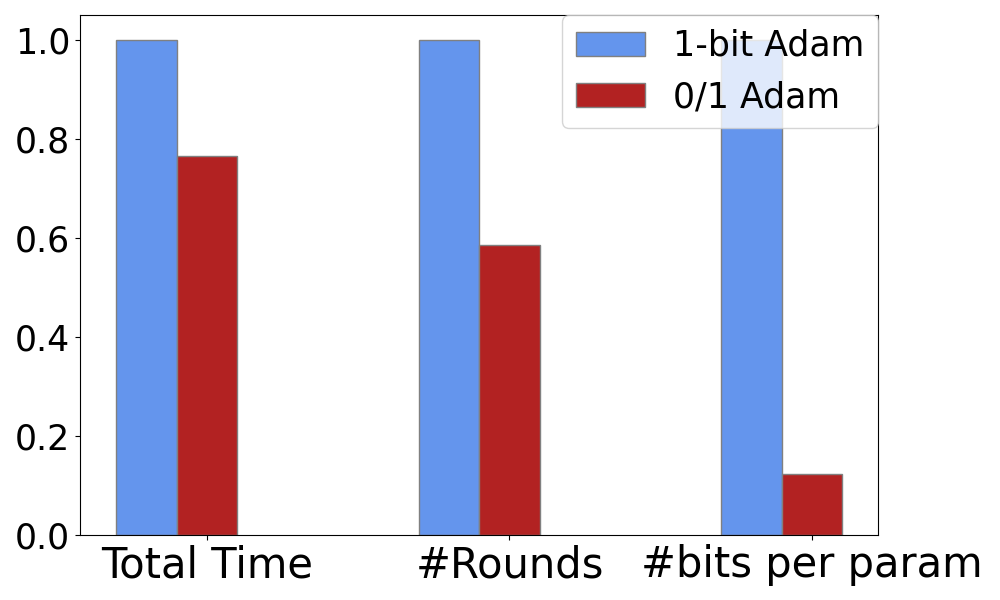
\includegraphics[width=0.31\textwidth]{./sections/figure/reduction_gpt.png}
  \caption{Reduction on number of bits per parameter used and number of communication rounds in different tasks. Note that the communication round numbers are normalized due to scale difference in different tasks.}%The right most figure specifies normalized numbers for the three metrics on GPT-2 (from left to right, with the order of 1-bit Adam/{\myalgo}) are: 34.52/26.29 hours, 300K/175K rounds, 5.0/0.61 bits, respectively.}
  \label{exp:fig:data_volume}
\end{figure}

\begin{figure}[t!]
  \centering
  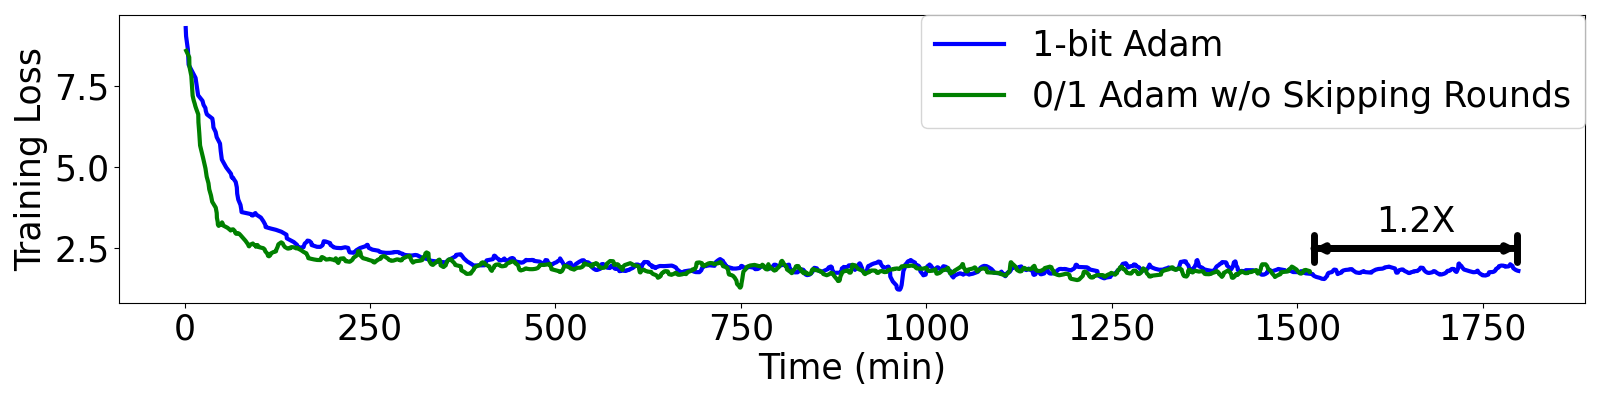
\includegraphics[width=0.49\textwidth]{./sections/figure/verify_v2_bbase.png}
  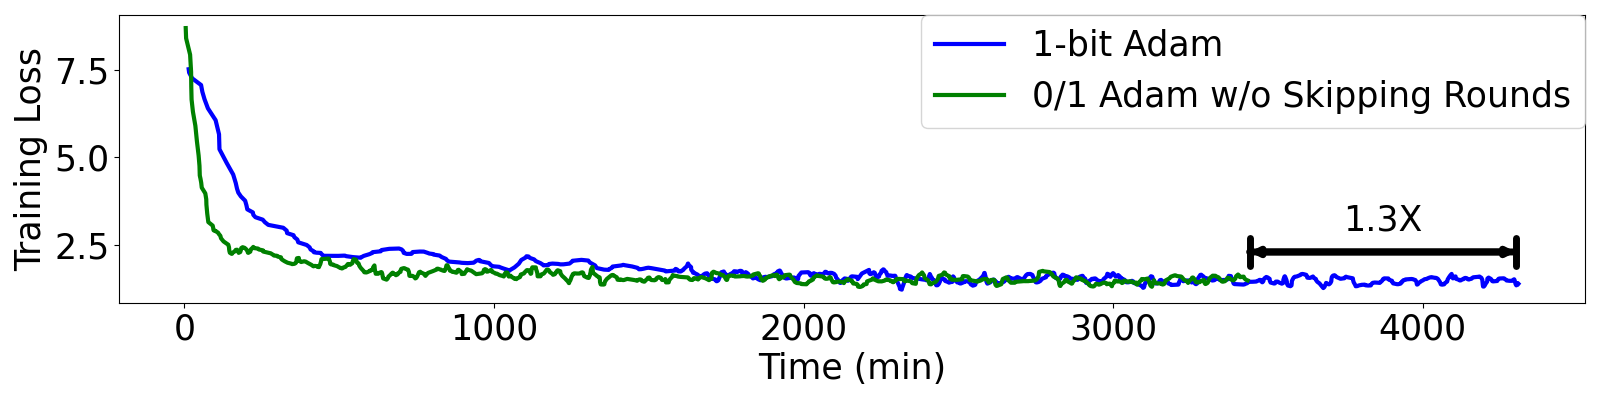
\includegraphics[width=0.49\textwidth]{./sections/figure/verify_v2_blarge.png}
  \caption{Evaluation BERT-Base/Large pretraining throughput using {\myalgo} without communication rounds skipping. Comparing with Figure~\ref{exp:fig:data_volume} and \ref{exp:fig:convergence}, local steps breaks the barrier on the performance gain.}
  \label{exp:fig:verify_v2}
\end{figure}

\subsection{Training Throughput Analysis}
Figure~\ref{exp:fig:throughput} summarizes the throughput results on different tasks and different clusters. We observe that {\myalgo} can consistently outperform baselines in all settings.
It is also worth mentioning that {\myalgo} on Ethernet (2.7 Gbps effective bandwidth, 4 GPUs per node) is able to achieve comparable throughput as 1-bit Adam on InfiniBand (near 100 Gbps effective bandwidth, 8 GPUs per node), as shown in the red line in Figure~\ref{exp:fig:throughput:bertlarge:eth} and the blue line in Figure~\ref{exp:fig:throughput:bertlarge:ib}, which demonstrates {\myalgo} further removes the redundancy in communication effectively that exceeds the hardware barrier.

\textbf{Communication reduction and the role of local steps.}
To better understand the importance and effect of local steps, we additionally run a special case of {\myalgo} where we keep the same policy of $\mathcal{T}_{\*v}$ but use $\mathcal{T}_{\*u}=\{0, \cdots, T-1\}$. This special version of {\myalgo} does not skip rounds but use the same variance freezing policy. We plot the data volume usage and throughput results in Figure~\ref{exp:fig:data_volume} and \ref{exp:fig:verify_v2}, respectively. We see that although no local steps suffice to reduce the data volume overhead from 1-bit Adam towards 1-bit-per-parameter in general, the throughput improvement is limited compared to Figure~\ref{exp:fig:convergence}.